\section{Wizard Spells}



\subsection{0-Level Wizard Spells (Cantrips)}

\subsubsection{Abjuration}
	\spellList{Resistance}: Subject gains +1 on saving throws.

\subsubsection{Conjuration}
	\spellList{Acid Splash}: Orb deals 1d3 acid damage.

\subsubsection{Divination}
	\spellList{Detect Poison}: Detects poison in one creature or small object.

	\spellList{Detect Magic}: Detects spells and magic items within 18 m.

	\spellList{Read Magic}: Read scrolls and spellbooks.

	\spellList{Slave Scent}: Divines target's social class. %%

\subsubsection{Enchantment}
	\spellList{Daze}: Humanoid creature of 4 HD or less loses next action.

\subsubsection{Evocation}
	\spellList{Dancing Lights}: Creates torches or other lights.

	\spellList{Flare}: Dazzles one creature ($-1$ on attack rolls).

	\spellList{Light}: Object shines like a torch.

	\spellList{Ray of Frost}: Ray deals 1d3 cold damage.

\subsubsection{Illusion}
	\spellList{Ghost Sound}: Figment sounds.

\subsubsection{Necromancy}
	\spellList{Disrupt Undead}: Deals 1d6 damage to one undead.

	\spellList{Touch of Fatigue}: Touch attack fatigues target.

\subsubsection{Transmutation}
	\spellList{Mage Hand}: 2-kg telekinesis.

	\spellList{Mending}: Makes minor repairs on an object.

	\spellList{Message}: Whispered conversation at distance.

	\spellList{Open/Close}: Opens or closes small or light things.

\subsubsection{Universal}
	\spellList{Arcane Mark}: Inscribes a personal rune (visible or invisible).

	\spellList{Prestidigitation}: Performs minor tricks.



\subsection{1st-Level Wizard Spells}

\subsubsection{Abjuration}
	\spellList{Alarm}: Wards an area for 2 hours/level.

	\spellList{Endure Elements}: Exist comfortably in hot or cold environments.

	\spellList{Hold Portal}: Holds door shut.

	\noindent\textit{\hyperref[spell:Protection from Chaos]{Protection from Chaos}/\hyperref[spell:Protection from Evil]{Evil}/\hyperref[spell:Protection from Good]{Good}/\hyperref[spell:Protection from Law]{Law}}: +2 to AC and saves, counter mind control, hedge out elementals and outsiders.

	\spellList{Shield}: Invisible disc gives +4 to AC, blocks magic missiles.

\subsubsection{Conjuration}
	\spellList{Cooling Canopy}: Summons a cloud to provide shade and prevent dehydration. %%

	\spellList{Grease}: Makes 3-m square or one object slippery.

	\spellList{Mage Armor}: Gives subject +4 armor bonus.

	\spellList{Mount}: Summons riding horse for 2 hours/level.

	\spellList{Obscuring Mist}: Fog surrounds you.

	\spellList{Summon Monster I}: Calls extraplanar creature to fight for you.

	\spellList{Unseen Servant}: Invisible force obeys your commands.

\subsubsection{Divination}
	\spellList{Comprehend Languages}: You understand all spoken and written languages.

	\spellList{Detect Secret Doors}: Reveals hidden doors within 18 m.

	\spellList{Detect Undead}: Reveals undead within 18 m.

	\spellList{Identify}\textsuperscript{M}: Determines properties of magic item.

	\spellList{True Strike}: +20 on your next attack roll.

\subsubsection{Enchantment}
	\spellList{Charm Person}: Makes one person your friend.

	\spellList{Hypnotism}: Fascinates 2d4 HD of creatures.

	\spellList{Sleep}: Puts 4 HD of creatures into magical slumber.

\subsubsection{Evocation}
	\spellList{Burning Hands}: 1d4/level fire damage (max 5d4).

	\spellList{Floating Disk}: Creates 1-m-diameter horizontal disk that holds 50 kg/level.

	\spellList{Magic Missile}: 1d4+1 damage; +1 missile per two levels above 1st (max 5).

	\spellList{Shocking Grasp}: Touch delivers 1d6/level electricity damage (max 5d6).

\subsubsection{Illusion}
	\spellList{Color Spray}: Knocks unconscious, blinds, and/or stuns weak creatures.

	\spellList{Disguise Self}: Changes your appearance.

	\spellList{Illusory Talent}: Provides the appearance of skill. %%

	\spellList{Magic Aura}: Alters object's magic aura.

	\spellList{Silent Image}: Creates minor illusion of your design.

	\spellList{Ventriloquism}: Throws voice for 1 min./level.

\subsubsection{Necromancy}
	\spellList{Cause Fear}: One creature of 5 HD or less flees for 1d4 rounds.

	\spellList{Chill Touch}: One touch/level deals 1d6 damage and possibly 1 Str damage.

	\spellList{Ray of Enfeeblement}: Ray deals 1d6 +1 per two levels Str damage.

\subsubsection{Transmutation}
	\spellList{Animate Rope}: Makes a rope move at your command.

	\spellList{Enlarge Person}: Humanoid creature doubles in size.

	\spellList{Erase}: Mundane or magical writing vanishes.

	\spellList{Expeditious Retreat}: Your speed increases by 9 m.

	\spellList{Feather Fall}: Objects or creatures fall slowly.

	\spellList{Jump}: Subject gets bonus on \skill{Jump} checks.

	\spellList{Magic Weapon}: Weapon gains +1 bonus.

	\spellList{Reduce Person}: Humanoid creature halves in size.



\subsection{2nd-Level Wizard Spells}

\subsubsection{Abjuration}
	\spellList{Arcane Lock}\textsuperscript{M}: Magically locks a portal or chest.

	\spellList{Backlash}: 1d6+1 damage/2 levels to defilers. %%

	\spellList{Eye of the Storm}: Protects 9-m radius from effects of storm for 1 hour/level.%%

	\spellList{Obscure Object}: Masks object against scrying.

	\spellList{Protection from Arrows}: Subject immune to most ranged attacks.

	\spellList{Resist Energy}: Ignores first 10 (or more) points of damage/attack from specified energy type.

\subsubsection{Conjuration}
	\spellList{Acid Arrow}: Ranged touch attack; 2d4 damage for 1 round +1 round/three levels.

	\spellList{Fog Cloud}: Fog obscures vision.

	\spellList{Glitterdust}: Blinds creatures, outlines invisible creatures.

	\spellList{Summon Monster II}: Calls extraplanar creature to fight for you.

	\spellList{Summon Swarm}: Summons swarm of bats, rats, or spiders.

	\spellList{Web}: Fills 6-m-radius spread with sticky spiderwebs.

\subsubsection{Divination}
	\spellList{Detect Thoughts}: Allows ``listening'' to surface thoughts.

	\spellList{Footsteps of the Quarry}: Track a specific creature or person. %%

	\spellList{Locate Object}: Senses direction toward object (specific or type).

	\spellList{See Invisibility}: Reveals invisible creatures or objects.

\subsubsection{Enchantment}
	\spellList{Daze Monster}: Living creature of 6 HD or less loses next action.

	\spellList{Hideous Laughter}: Subject loses actions for 1 round/level.

	\spellList{Touch of Idiocy}: Subject takes 1d6 points of Int, Wis, and Cha damage.

	\spellList{Wakefulness}: Target can postpone sleep. %%

\subsubsection{Evocation}
	\spellList{Cerulean Shock}: Imbue target with harmful static electricity. %%

	\spellList{Continual Flame}\textsuperscript{M}: Makes a permanent, heatless torch.

	\spellList{Darkness}: 6-m radius of supernatural shadow.

	\spellList{Flaming Sphere}: Creates rolling ball of fire, 2d6 damage, lasts 1 round/level.

	\spellList{Gust of Wind}: Blows away or knocks down smaller creatures.

	\spellList{Scorching Ray}: Ranged touch attack deals 4d6 fire damage, +1 ray/four levels (max 3).

	\spellList{Shatter}: Sonic vibration damages objects or crystalline creatures.

\subsubsection{Illusion}
	\spellList{Blur}: Attacks miss subject 20\% of the time.

	\spellList{Hypnotic Pattern}: Fascinates (2d4 + level) HD of creatures.

	\spellList{Invisibility}: Subject is invisible for 1 min./level or until it attacks.

	\spellList{Magic Mouth}\textsuperscript{M}: Speaks once when triggered.

	\spellList{Magic Trick}\textsuperscript{F}: Conceal your spellcasting. %%

	\spellList{Minor Image}: As \spell{silent image}, plus some sound.

	\spellList{Mirror Image}: Creates decoy duplicates of you (1d4 +1 per three levels, max 8).

	\spellList{Misdirection}: Misleads divinations for one creature or object.

	\spellList{Phantom Trap}\textsuperscript{M}: Makes item seem trapped.

\subsubsection{Necromancy}
	\spellList{Blindness/Deafness}: Makes subject blinded or deafened.

	\spellList{Command Undead}: Undead creature obeys your commands.

	\spellList{Death Mark}: Target becomes sickened. %%

	\spellList{False Life}: Gain 1d10 temporary hp +1/level (max +10).

	\spellList{Ghoul Touch}: Paralyzes one subject, which exudes stench that makes those nearby sickened.

	\spellList{Scare}: Panics creatures of less than 6 HD.

	\spellList{Spectral Hand}: Creates disembodied glowing hand to deliver touch attacks.

	\spellList{Sting of the Gold Scorpion}: Enlivens scorpion barb to strike with poison of real scorpion once. %%

\subsubsection{Transmutation}
	\spellList{Alter Self}: Assume form of a similar creature.

	\spellList{Bear's Endurance}: Subject gains +4 to Con for 1 min./level.

	\spellList{Boneharden}: Hardens bone, making weapons stronger and impairing living beings. %%

	\spellList{Bull's Strength}: Subject gains +4 to Str for 1 min./level.

	\spellList{Cat's Grace}: Subject gains +4 to Dex for 1 min./level.

	\spellList{Darkvision}: See 18 m in total darkness.

	\spellList{Eagle's Splendor}: Subject gains +4 to Cha for 1 min./level.

	\spellList{Fox's Cunning}: Subject gains +4 Int for 1 min./level.

	\spellList{Knock}: Opens locked or magically sealed door.

	\spellList{Levitate}: Subject moves up and down at your direction.

	\spellList{Owl's Wisdom}: Subject gains +4 to Wis for 1 min./level.

	\spellList{Pyrotechnics}: Turns fire into blinding light or choking smoke.

	\spellList{Rope Trick}: As many as eight creatures hide in extradimensional space.

	\spellList{Sandstone}: Touch turns sand into sandstone. %%

	\spellList{Spider Climb}: Grants ability to walk on walls and ceilings.

	\spellList{Whispering Wind}: Sends a short message 1.5 kg/level.



\subsection{3rd-Level Wizard Spells}

\subsubsection{Abjuration}
	\spellList{Conservation}\textsuperscript{M}: Protect the land from defilement. %%

	\spellList{Dispel Magic}: Cancels magical spells and effects.

	\spellList{Explosive Runes}: Deals 6d6 damage when read.

	\noindent\textit{\hyperref[spell:Magic Circle against Chaos]{Magic Circle against Chaos}/\hyperref[spell:Magic Circle against Evil]{Evil}/\hyperref[spell:Magic Circle against Good]{Good}/\hyperref[spell:Magic Circle against Law]{Law}}: As \emph{protection} spells, but 3-m radius and 10 min./level.

	\spellList{Nondetection}\textsuperscript{M}: Hides subject from divination, scrying.

	\spellList{Protection from Energy}: Absorb 12 points/level of damage from one kind of energy.

\subsubsection{Conjuration}
	\spellList{Phantom Steed}: Magic horse appears for 1 hour/level.

	\spellList{Sepia Snake Sigil}\textsuperscript{M}: Creates text symbol that immobilizes reader.

	\spellList{Sleet Storm}: Hampers vision and movement.

	\spellList{Stinking Cloud}: Nauseating vapors, 1 round/level.

	\spellList{Summon Monster III}: Calls extraplanar creature to fight for you.

\subsubsection{Divination}
	\spellList{Arcane Sight}: Magical auras become visible to you.

	\spellList{Clairaudience/Clairvoyance}\textsuperscript{F}: Hear or see at a distance for 1 min./level.

	\spellList{Telepathic Bond, Lesser}: As \spell{telepathic bond}, but you and one other creature.

	\spellList{Tongues}: Speak any language.

\subsubsection{Enchantment}
	\spellList{Dedication}: Allows target to avoid sleep, consume half food and water, and +1 to attack, damage, saves, ability, and skill checks while pursuing a specified task. %%

	\spellList{Deep Slumber}: Puts 10 HD of creatures to sleep.

	\spellList{Heroism}: Gives +2 bonus on attack rolls, saves, skill checks.

	\spellList{Hold Person}: Paralyzes one humanoid for 1 round/level.

	\spellList{Rage}: Subjects gains +2 to Str and Con, +1 on Will saves, $-2$ to AC.

	\spellList{Suggestion}: Compels subject to follow stated course of action.

\subsubsection{Evocation}
	\spellList{Clear-river}: Blows away or knocks creatures.

	\spellList{Daylight}: 18-m radius of bright light.

	\spellList{Fireball}: 1d6 damage per level, 6-m radius.

	\spellList{Lightning Bolt}: Electricity deals 1d6/level damage.

	\spellList{Tiny Hut}: Creates shelter for ten creatures.

	\spellList{Wind Wall}: Deflects arrows, smaller creatures, and gases.

\subsubsection{Illusion}
	\spellList{Displacement}: Attacks miss subject 50\%.

	\spellList{Illusory Script}\textsuperscript{M}: Only intended reader can decipher.

	\spellList{Invisibility Sphere}: Makes everyone within 3 m invisible.

	\spellList{Major Image}: As \spell{silent image}, plus sound, smell and thermal effects.

\subsubsection{Necromancy}
	\spellList{Boneclaw's Cut}\textsuperscript{F}: Deals damage that continues to cause bleeding damage. %%

	\spellList{Death Whip}\textsuperscript{F}: Whip deals temporary Strength damage. %%

	\spellList{Gentle Repose}: Preserves one corpse.

	\spellList{Halt Undead}: Immobilizes undead for 1 round/level.

	\spellList{Ray of Exhaustion}: Ray makes subject exhausted.

	\spellList{Vampiric Touch}: Touch deals 1d6/two levels damage; caster gains damage as hp.

\subsubsection{Transmutation}
	\spellList{Blink}: You randomly vanish and reappear for 1 round/level.

	\spellList{Flame Arrow}: Arrows deal +1d6 fire damage.

	\spellList{Fly}: Subject flies at speed of 18 m.

	\spellList{Gaseous Form}: Subject becomes insubstantial and can fly slowly.

	\spellList{Haste}: One creature/level moves faster, +1 on attack rolls, AC, and Reflex saves.

	\spellList{Keen Edge}: Doubles normal weapon's threat range.

	\spellList{Magic Weapon, Greater}: +1/four levels (max +5).

	\spellList{Sand Pit}: Excavates sand in a 9 m wide and 15 m deep cone. %%

	\spellList{Secret Page}: Changes one page to hide its real content.

	\spellList{Shrink Item}: Object shrinks to one-sixteenth size.

	\spellList{Slow}: One subject/level takes only one action/round, $-1$ to AC, reflex saves, and attack rolls.

	% \spellList{Water Breathing}: Subjects can breathe underwater.
	\spellList{Worm's Breath}: Subjects can breathe underwater, in silt or earth. %%

	\spellList{Zombie Berry}: Enchants 1d4 berries to act like a berry from the zombie plant. %%



\subsection{4th-Level Wizard Spells}

\subsubsection{Abjuration}
	\spellList{Dimensional Anchor}: Bars extradimensional movement.

	\spellList{Fire Trap}\textsuperscript{M}: Opened object deals 1d4 damage +1/level.

	\spellList{Globe of Invulnerability, Lesser}: Stops 1st- through 3rd-level spell effects.

	\spellList{Remove Curse}: Frees object or person from curse.

	\spellList{Stoneskin}\textsuperscript{M}: Ignore 10 points of damage per attack.

\subsubsection{Conjuration}
	\spellList{Black Tentacles}: Tentacles grapple all within 6 m spread.

	\spellList{Dimension Door}: Teleports you short distance.

	\spellList{Minor Creation}: Creates one cloth or wood object.

	\spellList{Secure Shelter}: Creates sturdy cottage.

	\spellList{Solid Fog}: Blocks vision and slows movement.

	\spellList{Summon Monster IV}: Calls extraplanar creature to fight for you.

\subsubsection{Divination}
	\spellList{Arcane Eye}: Invisible floating eye moves 9 m./round.

	\spellList{Detect Scrying}: Alerts you of magical eavesdropping.

	\spellList{Locate Creature}: Indicates direction to familiar creature.

	\spellList{Mage Seeker}\textsuperscript{F}: Locate nearby wizard. %%

	\spellList{Scrying}\textsuperscript{F}: Spies on subject from a distance.

\subsubsection{Enchantment}
	\spellList{Charm Monster}: Makes monster believe it is your ally.

	\spellList{Confusion}: Subjects behave oddly for 1 round/level.

	\spellList{Crushing Despair}: Subjects take $-2$ on attack rolls, damage rolls, saves, and checks.

	\spellList{Geas, Lesser}: Commands subject of 7 HD or less.

	\spellList{Gloomcloud}\textsuperscript{M}: Make one creature despair.

\subsubsection{Evocation}
	\spellList{Dweomer of Transference}: Convert spellcasting into psionic power points.

	\spellList{Fire Shield}: Creatures attacking you take fire damage; you're protected from heat or cold.

	\spellList{Ice Storm}: Hail deals 5d6 damage in cylinder 12 m across.

	\spellList{Resilient Sphere}: Force globe protects but traps one subject.

	\spellList{Sand Spray}: Sprays sand or silt as an area attack. %%

	\spellList{Shout}: Deafens all within cone and deals 5d6 sonic damage.

	\spellList{Wall of Fire}: Deals 2d4 fire damage out to 3 m and 1d4 out to 6 m. Passing through wall deals 2d6 damage +1/level.

	\spellList{Wall of Ice}: Ice plane creates wall with 15 hp +1/level, or hemisphere can trap creatures inside.

\subsubsection{Illusion}
	\spellList{Hallucinatory Terrain}: Makes one type of terrain appear like another (field into forest, or the like).

	\spellList{Illusory Wall}: Wall, floor, or ceiling looks real, but anything can pass through.

	\spellList{Invisibility, Greater}: As \spell{invisibility}, but subject can attack and stay invisible.

	\spellList{Phantasmal Killer}: Fearsome illusion kills subject or deals 3d6 damage.

	\spellList{Rainbow Pattern}: Lights fascinate 24 HD of creatures.

	\spellList{Shadow Conjuration}: Mimics conjuration below 4th level, but only 20\% real.

\subsubsection{Necromancy}
	\spellList{Animate Dead}\textsuperscript{M}: Creates undead skeletons and zombies.

	\spellList{Bestow Curse}: $-6$ to an ability score; $-4$ on attack rolls, saves, and checks; or 50\% chance of losing each action.

	\spellList{Claws of the Tembo}: Deals 1d6 Str damage and transfers hp. %%

	\spellList{Contagion}: Infects subject with chosen disease.

	\spellList{Enervation}: Subject gains 1d4 negative levels.

	\spellList{Fear}: Subjects within cone flee for 1 round/level.

	\spellList{Ghostfire}: Kills 2 HD/level of creatures (max 40 HD). %%

	\spellList{Touch the Black}\textsuperscript{M}: Cold deals 1d6 damage per level, 12-m radius. %%

\subsubsection{Transmutation}
	\spellList{Enlarge Person, Mass}: Enlarges several creatures.

	\spellList{Mnemonic Enhancer}\textsuperscript{F}: Prepares extra spells or retains one just cast.

	\spellList{Polymorph}: Gives one willing subject a new form.

	\spellList{Reduce Person, Mass}: Reduces several creatures.

	\spellList{Stone Shape}: Sculpts stone into any shape.



\subsection{5th-Level Wizard Spells}

\subsubsection{Abjuration}
	\spellList{Break Enchantment}: Frees subjects from enchantments, alterations, curses, and petrification.

	\spellList{Dismissal}: Forces a creature to return to native plane.

	\spellList{Mage's Private Sanctum}: Prevents anyone from viewing or scrying an area for 24 hours.

	\spellList{Psychic Turmoil}: Invisible field leeches psionic power points away.

\subsubsection{Conjuration}
	\spellList{Cerulean Hail}: A hailstorm appears and does 3d8 damage and causes less than 10 HD creatures to flee. %%

	\spellList{Cloudkill}: Kills 3 HD or less; 4$-6$ HD save or die, 6+ HD take Con damage.

	\spellList{Mage's Faithful Hound}: Phantom dog can guard, attack.

	\spellList{Major Creation}: As \spell{minor creation}, plus stone and metal.

	\spellList{Planar Binding, Lesser}: Traps extraplanar creature of 6 HD or less until it performs a task.

	\spellList{Secret Chest}\textsuperscript{F}: Hides expensive chest on Ethereal Plane; you retrieve it at will.

	\spellList{Summon Monster V}: Calls extraplanar creature to fight for you.

	\spellList{Teleport}: Instantly transports you as far as 150 km/level.

	\spellList{Wall of Stone}: Creates a stone wall that can be shaped.

\subsubsection{Divination}
	\spellList{Contact Other Plane}: Lets you ask question of extraplanar entity.

	\spellList{Prying Eyes}: 1d4 +1/level floating eyes scout for you.

	\spellList{Telepathic Bond}: Link lets allies communicate.

\subsubsection{Enchantment}
	\spellList{Dominate Person}: Controls humanoid telepathically.

	\spellList{Feeblemind}: Subject's Int and Cha drop to 1.

	\spellList{Hold Monster}: As \spell{hold person}, but any creature.

	\spellList{Mind Fog}: Subjects in fog get $-10$ to Wis and Will checks.

	\spellList{Scapegoat}\textsuperscript{M}: Put the blame on a nearby target. %%

	\spellList{Symbol of Sleep}\textsuperscript{M}: Triggered rune puts nearby creatures into catatonic slumber.

\subsubsection{Evocation}
	
	\spellList{Cone of Cold}: 1d6/level cold damage.
	
	\spellList{Interposing Hand}: Hand provides cover against one opponent.
	
	\spellList{Quietstorm}: Ranged touch attack deals 8d6 sonic damage. %%
	
	\spellList{Ragestorm}\textsuperscript{M}: Storm rains hail, winds and lightning. %%
	
	\spellList{Sending}: Delivers short message anywhere, instantly.

	\spellList{Skyfire}: Three exploding spheres each deal 1d6 bludgeoning damage and 3d6 fire damage. %%
	
	\spellList{Sparkrain}: Bolt dispels magical effects. %%
	
	\spellList{Wall of Force}: Wall is immune to damage.

\subsubsection{Illusion}
	\spellList{Dream}: Sends message to anyone sleeping.

	\spellList{False Vision}\textsuperscript{M}: Fools scrying with an illusion.

	\spellList{Mirage Arcana}: As \spell{hallucinatory terrain}, plus structures.

	\spellList{Nightmare}: Sends vision dealing 1d10 damage, fatigue.

	\spellList{Persistent Image}: As \spell{major image}, but no concentration required.

	\spellList{Seeming}: Changes appearance of one person per two levels.

	\spellList{Shadow Evocation}: Mimics evocation below 5th level, but only 20\% real.

\subsubsection{Necromancy}
	\spellList{Blight}: Withers one plant or deals 1d6/level damage to plant creature.

	\spellList{Magic Jar}\textsuperscript{F}: Enables possession of another creature.

	\spellList{Symbol of Pain}\textsuperscript{M}: Triggered rune wracks nearby creatures with pain.

	\spellList{Waves of Fatigue}: Several targets become fatigued.

\subsubsection{Transmutation}
	\spellList{Animal Growth}: One animal/two levels doubles in size.
	
	\spellList{Baleful Polymorph}: Transforms subject into harmless animal.
	
	\spellList{Fabricate}: Transforms raw materials into finished items.
	
	\spellList{Overland Flight}: You fly at a speed of 12 m and can hustle over long distances.
	
	\spellList{Passwall}: Creates passage through wood or stone wall.
	
	\spellList{Rangeblade}: Can strike with melee weapons at a distance. %%
	
	\spellList{Sand Trap}\textsuperscript{M}: You entrap an area of sand. %%
	
	\spellList{Sandflow}: You shift the location of sand dunes. %%
	
	\spellList{Telekinesis}: Moves object, attacks creature, or hurls object or creature.
	
	\spellList{Transmute Mud to Rock}: Transforms two 3-m cubes per level.
	
	\spellList{Transmute Rock to Mud}: Transforms two 3-m cubes per level.

\subsubsection{Universal}
	\spellList{Permanency}\textsuperscript{X}: Makes certain spells permanent.



\subsection{6th-Level Wizard Spells}

\subsubsection{Abjuration}
	\spellList{Antimagic Field}: Negates magic within 3 m.

	\spellList{Banish Tyr-Storm}\textsuperscript{F}: Repel a Tyr-storm. %%

	\spellList{Dispel Magic, Greater}: As \spell{dispel magic}, but +20 on check.

	\spellList{Globe of Invulnerability}: As \spell{lesser globe of invulnerability}, plus 4th-level spell effects.

	\spellList{Guards and Wards}: Array of magic effects protect area.

	\spellList{Repulsion}: Creatures can't approach you.

\subsubsection{Conjuration}
	\spellList{Acid Fog}: Fog deals acid damage.

	\spellList{Planar Binding}: As \spell{lesser planar binding}, but up to 12 HD.

	\spellList{Summon Monster VI}: Calls extraplanar creature to fight for you.

	\spellList{Summon Tyr-Storm}\textsuperscript{F}: Call a powerful Tyr-storm. %%

	\spellList{Wall of Iron}\textsuperscript{M}: 30 hp/four levels; can topple onto foes.

\subsubsection{Divination}
	\spellList{Analyze Dweomer}\textsuperscript{F}: Reveals magical aspects of subject.

	\spellList{Legend Lore}\textsuperscript{MF}: Lets you learn tales about a person, place, or thing.

	\spellList{Probe Thoughts}: Read subject's memories, one question/round.

	\spellList{True Seeing}\textsuperscript{M}: Lets you see all things as they really are.

\subsubsection{Enchantment}
	\spellList{Geas/Quest}: As \spell{lesser geas}, plus it affects any creature.

	\spellList{Heroism, Greater}: Gives +4 bonus on attack rolls, saves, skill checks; immunity to fear; temporary hp.

	\spellList{Suggestion, Mass}: As \spell{suggestion}, plus one subject/level.

	\spellList{Symbol of Persuasion}\textsuperscript{M}: Triggered rune charms nearby creatures.

\subsubsection{Evocation}
	\spellList{Chain Lightning}: 1d6/level damage; 1 secondary bolt/level each deals half damage.

	\spellList{Cleansing Flame}: 1d6/level fire damage (max 10d6). %%

	\spellList{Contingency}\textsuperscript{F}: Sets trigger condition for another spell.

	\spellList{Forceful Hand}: Hand pushes creatures away.

	\spellList{Freezing Sphere}: Freezes water or deals cold damage.

	\spellList{Groundflame}: Mist deals acid damage. %%

\subsubsection{Illusion}
	\spellList{Mislead}: Turns you invisible and creates illusory double.

	\spellList{Permanent Image}\textsuperscript{M}: Includes sight, sound, and smell.

	\spellList{Programmed Image}\textsuperscript{M}: As \spell{major image}, plus triggered by event.

	\spellList{Shadow Walk}: Step into shadow to travel rapidly.

	\spellList{Veil}: Changes appearance of group of creatures.

\subsubsection{Necromancy}
	\spellList{Circle of Death}\textsuperscript{M}: Kills 1d4/level HD of creatures.

	\spellList{Create Undead}\textsuperscript{M}: Creates ghouls, ghasts, mummies, or mohrgs.

	\spellList{Eyebite}: Target becomes panicked, sickened, and comatose.

	\spellList{Shroud of Darkness}\textsuperscript{M}: Imbue a cloak with protective qualities. %%

	\spellList{Symbol of Fear}\textsuperscript{M}: Triggered rune panics nearby creatures.

	\spellList{Undeath to Death}\textsuperscript{M}: Destroys 1d4/level HD of undead (max 20d4).

\subsubsection{Transmutation}
	% \spellList{Control Water}: Raises or lowers bodies of water.

	\spellList{Bear's Endurance, Mass}: As \spell{bear's endurance}, affects one subject/level.

	\spellList{Braxatskin}: Your skin hardens, granting armor bonus and damage reduction. %%

	\spellList{Bull's Strength, Mass}: As \spell{bull's strength}, affects one subject/ level.

	\spellList{Cat's Grace, Mass}: As \spell{cat's grace}, affects one subject/level.

	\spellList{Control Tides}: Raises, lowers, or parts bodies of water or silt. %%

	\spellList{Disintegrate}: Makes one creature or object vanish.

	\spellList{Eagle's Splendor, Mass}: As \spell{eagle's splendor}, affects one subject/level.

	\spellList{Flesh to Stone}: Turns subject creature into statue.

	\spellList{Fox's Cunning, Mass}: As \spell{fox's cunning}, affects one subject/ level.

	\spellList{Hardening}: Permanently increase by 1/two levels the hardness of an item.

	\spellList{Mage's Lucubration}: Recalls spell of 5th level or lower.

	\spellList{Mental Pinnacle}\textsuperscript{M}: You gain the mental powers of a psion.

	\spellList{Move Earth}: Digs trenches and build hills.

	\spellList{Owl's Wisdom, Mass}: As \spell{owl's wisdom}, affects one subject/ level.

	\spellList{Sands of Time}\textsuperscript{F}: Reverses or accelerates aging of a nonliving object. %%

	\spellList{Shining Sands}: Grains of sand rotate to reflect light where you wish it to go. %%

	\spellList{Stone to Flesh}: Restores petrified creature.

	\spellList{Transformation}\textsuperscript{M}: You gain combat bonuses.



\subsection{7th-Level Wizard Spells}

\subsubsection{Abjuration}
	\spellList{Banishment}: Banishes 2 HD/level of extraplanar creatures.

	\spellList{Psychic Turmoil, Greater}: As \spell{psychic turmoil}, but you gain power points as temporary hit points.

	\spellList{Sequester}: Subject is invisible to sight and scrying; renders creature comatose.

	\spellList{Spell Turning}: Reflect 1d4+6 spell levels back at caster.

\subsubsection{Conjuration}
	\spellList{Infestation}: Tiny parasites infest creatures within area. %%

	\spellList{Instant Summons}\textsuperscript{M}: Prepared object appears in your hand.

	\spellList{Mage's Magnificent Mansion}\textsuperscript{F}: Door leads to extradimensional mansion.

	\spellList{Phase Door}: Creates an invisible passage through wood or stone.

	\spellList{Plane Shift}\textsuperscript{F}: As many as eight subjects travel to another plane.

	\spellList{Summon Monster VII}: Calls extraplanar creature to fight for you.

	\spellList{Teleport, Greater}: As \spell{teleport}, but no range limit and no off-target arrival.

	\spellList{Teleport Object}: As \spell{teleport}, but affects a touched object.

\subsubsection{Divination}
	\spellList{Arcane Sight, Greater}: As \spell{arcane sight}, but also reveals magic effects on creatures and objects.

	\spellList{Scrying, Greater}: As \spell{scrying}, but faster and longer.

	\spellList{Vision}\textsuperscript{MX}: As \spell{legend lore}, but quicker and strenuous.

\subsubsection{Enchantment}
	\spellList{Hold Person, Mass}: As \spell{hold person}, but all within 9 m.

	\spellList{Insanity}: Subject suffers continuous confusion.

	\spellList{Power Word Blind}: Blinds creature with 200 hp or less.

	\spellList{Symbol of Stunning}\textsuperscript{M}: Triggered rune stuns nearby creatures.

\subsubsection{Evocation}
	\spellList{Delayed Blast Fireball}: 1d6/level fire damage; you can postpone blast for 5 rounds.

	\spellList{Forcecage}\textsuperscript{M}: Cube or cage of force imprisons all inside.

	\spellList{Grasping Hand}: Hand provides cover, pushes, or grapples.

	\spellList{Mage's Sword}\textsuperscript{F}: Floating magic blade strikes opponents.

	\spellList{Prismatic Spray}: Rays hit subjects with variety of effects.

\subsubsection{Illusion}
	\spellList{Invisibility, Mass}: As \spell{invisibility}, but affects all in range.

	\spellList{Project Image}: Illusory double can talk and cast spells.

	\spellList{Shadow Conjuration, Greater}: As \spell{shadow conjuration}, but up to 6th level and 60\% real.

	\spellList{Simulacrum}\textsuperscript{MX}: Creates partially real double of a creature.

\subsubsection{Necromancy}
	\spellList{Control Undead}: Undead don't attack you while under your command.
	
	\spellList{Finger of Death}: Kills one subject.
	
	\spellList{Gray Beckoning}: Summons zombies from the Gray. %%

	\spellList{Symbol of Weakness}\textsuperscript{M}: Triggered rune weakens nearby creatures.

	\spellList{Unliving Identity}\textsuperscript{MX}: Transform a zombie into a thinking 
	zombie. %%
	
	\spellList{Waves of Exhaustion}: Several targets become exhausted.

\subsubsection{Transmutation}
	\spellList{Control Weather}: Changes weather in local area.

	\spellList{Ethereal Jaunt}: You become ethereal for 1 round/level.

	\spellList{Reverse Gravity}: Objects and creatures fall upward.

	\spellList{Statue}: Subject can become a statue at will.

\subsubsection{Universal}
	\spellList{Limited Wish}\textsuperscript{X}: Alters reality---within spell limits.



\subsection{8th-Level Wizard Spells}

\subsubsection{Abjuration}
	\spellList{Dimensional Lock}: Teleportation and interplanar travel blocked for one day/level.

	\spellList{Mind Blank}: Subject is immune to mental/emotional magic and scrying.

	\spellList{Prismatic Wall}: Wall's colors have array of effects.

	\spellList{Protection from Spells}\textsuperscript{MF}: Confers +8 resistance bonus.

	\spellList{Protection from Time}\textsuperscript{MX}: Makes creature or object immune to aging for 1 month/2 levels. %%

\subsubsection{Conjuration}
	\spellList{Incendiary Cloud}: Cloud deals 4d6 fire damage/round.

	\spellList{Maze}: Traps subject in extradimensional maze.

	\spellList{Planar Binding, Greater}: As \spell{lesser planar binding}, but up to 18 HD.

	\spellList{Summon Monster VIII}: Calls extraplanar creature to fight for you.

	\spellList{Trap the Soul}\textsuperscript{MF}: Imprisons subject within gem.

\subsubsection{Divination}
	\spellList{Discern Location}: Reveals exact location of creature or object.

	\spellList{Moment of Prescience}: You gain insight bonus on single attack roll, check, or save.

	\spellList{Prying Eyes, Greater}: As \spell{prying eyes}, but eyes have \spell{true seeing}.

\subsubsection{Enchantment}
	\spellList{Antipathy}: Object or location affected by spell repels certain creatures.

	\spellList{Binding}\textsuperscript{M}: Utilizes an array of techniques to imprison a creature.

	\spellList{Charm Monster, Mass}: As \spell{charm monster}, but all within 9 m.

	\spellList{Demand}: As \spell{sending}, plus you can send suggestion.

	\spellList{Irresistible Dance}: Forces subject to dance.

	\spellList{Maddening Scream}: Subject has $-4$ AC, no shield, Reflex save on 20 only.

	\spellList{Power Word Stun}: Stuns creature with 150 hp or less.

	\spellList{Symbol of Insanity}\textsuperscript{M}: Triggered rune renders nearby creatures insane.

	\spellList{Sympathy}\textsuperscript{F}: Object or location attracts certain creatures.

\subsubsection{Evocation}
	\spellList{Clenched Fist}: Large hand provides cover, pushes, or attacks your foes.

	\spellList{Polar Ray}: Ranged touch attack deals 1d6/level cold damage.

	\spellList{Shout, Greater}: Devastating yell deals 10d6 sonic damage; stuns creatures, damages objects.

	\spellList{Sunburst}: Blinds all within 3 m, deals 6d6 damage.

	\spellList{Telekinetic Sphere}: As \spell{resilient sphere}, but you move sphere telekinetically.

\subsubsection{Illusion}
	\spellList{Scintillating Pattern}: Twisting colors confuse, stun, or render unconscious.

	\spellList{Screen}: Illusion hides area from vision, scrying.

	\spellList{Shadow Evocation, Greater}: As \spell{shadow evocation}, but up to 7th level and 60\% real.

\subsubsection{Necromancy}
	\spellList{Clone}\textsuperscript{MF}: Duplicate awakens when original dies.

	\spellList{Create Greater Undead}\textsuperscript{M}: Create shadows, wraiths, spectres, or devourers.

	\spellList{Horrid Wilting}: Deals 1d6/level damage within 9 m.

	\spellList{Symbol of Death}\textsuperscript{M}: Triggered rune slays nearby creatures.

\subsubsection{Transmutation}
	\spellList{Iron Body}: Your body becomes living iron.

	\spellList{Polymorph Any Object}: Changes any subject into anything else.

	\spellList{Temporal Stasis}\textsuperscript{M}: Puts subject into suspended animation.


\begin{figure*}[b!]
\centering
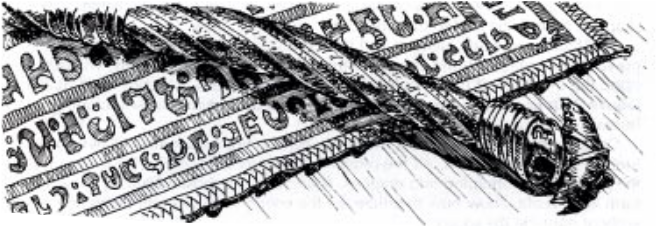
\includegraphics[width=\textwidth]{images/filler-1.png}
\WOTC
\end{figure*}


\subsection{9th-Level Wizard Spells}

\subsubsection{Abjuration}
	\spellList{Freedom}: Releases creature from imprisonment.

	\spellList{Imprisonment}: Entombs subject beneath the earth.

	\spellList{Mage's Disjunction}: Dispels magic, disenchants magic items.

	\spellList{Prismatic Sphere}: As \spell{prismatic wall}, but surrounds on all sides.

\subsubsection{Conjuration}
	\spellList{Gate}\textsuperscript{X}: Connects two planes for travel or summoning.

	\spellList{Gray Rift}: A hovering rift to the Gray bolsters undead. %%

	\spellList{Refuge}\textsuperscript{M}: Alters item to transport its possessor to you.

	\spellList{Summon Monster IX}: Calls extraplanar creature to fight for you.

	\spellList{Teleportation Circle}\textsuperscript{M}: Circle teleports any creature inside to designated spot.

\subsubsection{Divination}
	\spellList{Foresight}: ``Sixth sense'' warns of impending danger.

\subsubsection{Enchantment}
	\spellList{Dominate Monster}: As \spell{dominate person}, but any creature.

	\spellList{Hold Monster, Mass}: As \spell{hold monster}, but all within 9 m.

	\spellList{Power Word Kill}: Kills one creature with 100 hp or less.

\subsubsection{Evocation}
	\spellList{Crushing Hand}: Large hand provides cover, pushes, or crushes your foes.

	\spellList{Meteor Swarm}: Four exploding spheres each deal 6d6 fire damage.

	\spellList{Tempest}\textsuperscript{M}: Create an obliterating storm. %%

\subsubsection{Illusion}
	\spellList{Shades}: As \spell{shadow conjuration}, but up to 8th level and 80\% real.

	\spellList{Weird}: As \spell{phantasmal killer}, but affects all within 9 m.

\subsubsection{Necromancy}
	\spellList{Astral Projection}\textsuperscript{M}: Projects you and companions onto Astral Plane.

	\spellList{Energy Drain}: Subject gains 2d4 negative levels.

	\spellList{Pact of Darkness}\textsuperscript{M}: Exchange services with a shadow giant. %%

	\spellList{Soul Bind}\textsuperscript{F}: Traps newly dead soul to prevent resurrection.

	\spellList{Vampiric Youthfulness}: Increases your lifespan at the expense of another's. %%

	\spellList{Wail of the Banshee}: Kills one creature/level.

\subsubsection{Transmutation}
	\spellList{Etherealness}: Travel to Ethereal Plane with companions.

	\spellList{Magma Tunnel}: Tunnels through solid rock. %%

	\spellList{Shapechange}\textsuperscript{F}: Transforms you into any creature, and change forms once per round.

	\spellList{Time Stop}: You act freely for 1d4+1 rounds.

\subsubsection{Universal}
	\spellList{Wish}\textsuperscript{X}: As \spell{limited wish}, but with fewer limits.